
\section{Modelo}
Dado el conjunto de items I y la función de similitud \textbf{S}: IxI$\rightarrow$R[0;1]. El problema se puede representar como un grafo 
con peso en las aristas, en el cuál los vertices son los items y el peso de las aristas es la similitud entres estos.
\section{Problema}
El problema de obtener el conjunto de bundles que máximiza la función objetivo se puede considerar como un problema
de clusterización en el cual la calidad de los cluster esta dado por la cohesión de los items que lo componen y la
separación entre cluster con menos similitud.
Las diferencias con los problemas tipicos de clusterización son:
\begin{enumerate}
 \item La cantidad de items en un bundle esta limitada por el presupuesto.
 \item En el bundle no puede existir más de un item con el mismo atributo de complementaridad.
\end{enumerate}
\section{Función de similitud}
La similitud se emplea para comparar dos documentos y determinar que tan parecido sonentre si. La comparación se realiza en el \textit{modelo de espacio vectorial} donde los artículos se representan con vectores, en la que cada dimensión corresponde a un tópico. El valor del tópico del artículo en la base de datos, es el valor en el vector.\\
El artículo $a$ se representa con el vector $V_a = [v_1,v_2,...,v_n]$, donde $N$ es la cantidad de tópicos. Los vectores cumplen las siguientes propiedades:
\begin{enumerate}
 \item $v_i \leqslant 1$
 \item $\sum{v_i} = 1$
\end{enumerate}

Con los vectores es posible calcular el coeficiente de similitud a través de la función $ S (V_i, V_j)$ la cual refleja el grado de similitud de los pesos de los tópicos correspondientes. Existen varias medidas de similitud, En este trabajo se utilizó una de las más utilizadas que es la medida de similitud basada en el ángulo de los vectores.\\
En la medida de similitud del coseno la dirección de los vectores es lo que se utiliza para determinar que tan parecidos son entre si. Cuanto más parecido sean los documentos el ángulo de los vectores se acerca a cero. Siendo que dos vectores con identica distribución de los términos, el ángulo es cero, produciendo la máxima medida de similitud.\\
Conforme a \cite{newSimilarity} el ángulo de dos vectores proporcionales tienen la misma dirección con lo que el ángulo es cero. Entonces estos vectores son exactamente similares en cuanto a la medida de similitud basada en el ángulo. Esta medida no considera el peso de cada tópico. Por lo tanto no diferencia entre un articulo profesional y un articulo de un diario que cubre el mismo tópico. Esta debilidad de la medida basada en el ángulo no interfiere en este trabajo, por las propiedades de los vectores los documentos. Porque los documentos con tópicos similares se representan con vectores que se encuentran muy cerca en el espacio euclediano.

Dado los vectores $V_i$ y $V_j$ la función de similitud basada en el ángulo se obtiene por la definición del producto escalar.\\
\begin{equation} \label{eq:angulovectorial}
\cos(\theta) =  \dfrac{\overrightarrow{U} . \overrightarrow{V}}{\overrightarrow{\lVert V\lVert}.\overrightarrow{\lVert U\lVert}}
\end{equation}

Como los componentes de todos los vectores son mayor o igual a cero se obtien que $0\leq\cos(\theta)\geq1$. Que corresponde con la función de similitud.

\begin{figure}[H]
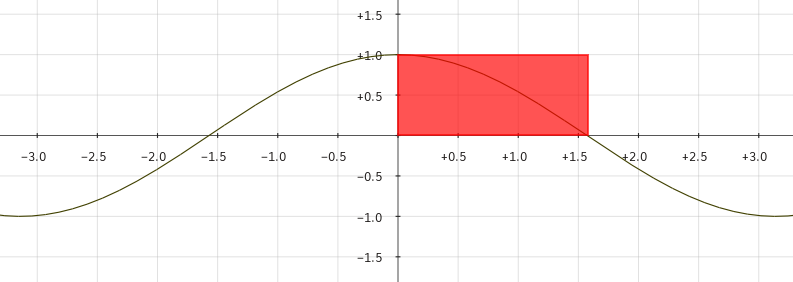
\includegraphics[width=0.8\textwidth]{img/coseno.png}
\caption{Comportamiento de la función $\cos$. En rojo la región que involucra los resutlados de la función de similitud}
\label{bus:img-coseno}
\end{figure}


\section{Resolución}
Encontrar una solución al problema planteado es reducible 

El algoritmo que se utilizó para obtener las soluciones es \texttt{Produce-and-Choose}, cuenta con 
dos fases.
En la primer fase se generan cierta cantidad de bundles, e la fase siguiente se seleccionan los 
bundles que serán parte de la solución.\\
A continuación se explican los algoritmos utilizados para cada fase.
\section{Generación de bundles}
Dado un conjunto de papers el objetivo es generar clusters en los cuales los papers suficientemente 
similares pertenezcan al mismo cluster y en cluster distintos los disímiles. Cuanto mayor es la 
similitud en el cluster (intra) y mayor la diferencia entre los cluster (inter) es mejor la 
clusterización.\\
Definir como se constituye un cluster es complejo. Por ejemplo para los 20 puntos que se muestran a 
continuación existen tres (o más) formas de clusterizar que son validas. Entonces la mejor 
definición depende del tipo de dato y del resultado esperado.

\begin{figure}[H]
  \centering
    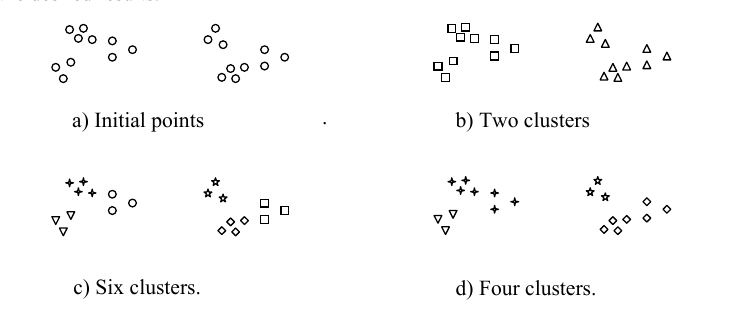
\includegraphics[width=0.8\textwidth]{img/howToCluster.png}
  \caption{Agregar descripcion}
  \label{res:img-howToCluster}
\end{figure}

En la clusterización para Composite Retrival, la definición es generar cluster máximizando el costo que esta acotado por el budget.
Ya que lo esperado es obtener cluster que utilicen el máximo del presupuesto.\\

El problema de la clusterización es NP-hard (agregar ref, explicar problema de clusterizacion),
por lo que se utilizaron dos técnicas ya conocidas para aproximarse a una solución.\\
La principal diferencia entre las estrategias de clusterización es entre la jerárquica y de 
partición.\\
La primer técnica produce un árbol de particiones, la raíz es un cluster que contiene todos los items
y las hojas son clusters con un único ítem. Cada nivel intermedio, puede ser visto, como la 
combinación entre dos clusters del nivel inferior inmediato. Mientras que la segunda genera solo un 
nivel de las particiones de los items de una vez.\\ 
Se implementaron las dos técnicas para la clusterización jerárquica con el algoritmo
Hierarchical clustering y la de partición con Bundles One-By-One.\\

\subsection{Bundles One-By-One}
El método \texttt{BOBO-x} esta inspirado en k-nn. Consiste en cada paso seleccionar, de manera azarosa, un item del conjunto de pivotes (en el inicio este conjunto contiente todos los items),
con el que se genera un bundle valido a al rededor de este. En el caso de que el intra del bundle sea bueno se agrga al conjunto de candidatos de bundle.
La iteración finaliza cuando se generan la cantidad de candidatos definidos en el parámetro $x$ o cuando el conjunto de bundles es vacío. El caso de que $x$ sea 'Ex' todos los 
items son pivotes.\\
Para generar el bundle a partir del pivote, se realiza de manera golosa de eligiendo en cada iteración el item que
máximiza el intra y que cumple con las resticciones.\\
\subsection{Hierarchical clustering}
La heurística Hierarchical clustering \texttt{HAC} comienza con tantos clusters como cantidad de elementos, cada uno está 
conformado por un solo ítem y en cada paso se unen los dos clusters más cercanos que respetan las restricciones. 
Para ello se define la función de distancia para los items $u$ y $v$ como:\\
\begin{equation}
d_{1}(u,v) = 1 - s(u, v)
\end{equation}

Con la función de distancia $d_{1}$ en la clusterización se generan los cluster lo más cohesivos posibles,
En la figura 1 se observa que el algoritmo selecciona los items más cercanos. En las búsquedas que 
se realizan en ``Composite ...''\cite{compositeRetrival} se tiene el parámetro $\gamma$ que indica 
que tipo de resultado es el esperado. 

\begin{figure}[H]
  \centering
    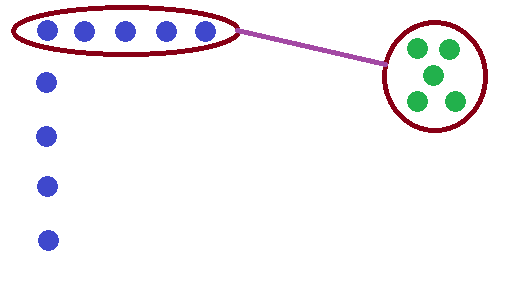
\includegraphics[width=0.3\textwidth]{img/cluster2.png}
  \caption{Selección de bundles usando $d_{1}$}
  \label{res:img-usingEfficientHAC}
\end{figure}

En caso de que el $\gamma$ sea pequeño, la 
clusterización esperada para la misma instancia es la que se visualiza en la imágen 2, clusters no 
tan cohesivos pero más variados. Por lo que se define una función de distancia que considera el 
$\gamma$.\\
\begin{equation}
d2(u,v) = 1 - FO(\{u\} \cup \{v\})
\end{equation}
Donde $FO$ es la función definida en \eqref{eq:fnObj} \\

\begin{figure}[H]
  \centering
    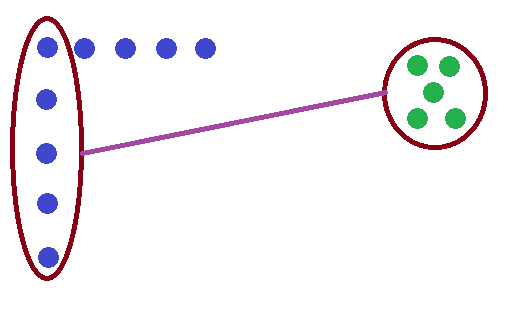
\includegraphics[width=0.3\textwidth]{img/cluster1.png}
  \caption{Selección de bundles usando $d_{2}$}
  \label{res:img-usingSingleHAC}
\end{figure}

Para la distancia $d_{1}$ se implementó el algoritmo \texttt{EfficientHAC} que es tiene una 
complejidad $\mathcal{O}(n^{2})$, mientras que para $d_{2}$ el algoritmo es \texttt{SingleHAC} que 
la complejidad es $\mathcal{O}(n^{2} * \ln{n})$. Según se demostró en el capítulo 17 de 
\cite{informationRetrival}


\section{Selección de bundles}
Al finalizar la producción de bundles, se deben seleccionar los $k$ bundles para la solución.
El problema de seleccionar los bundles que maximizan la función objetivo, se traduce en 
encontrar en el grafo G el k-subgrafo de mayor peso de nodos y aristas.

Se implementó el algoritmo que propone ``Composite ...''\cite{compositeRetrival} que transforma el 
grafo G en el grafo G', con los mismos nodos y aristas, redefiniendo el peso de las aristas con la 
función:\\

\begin{equation}
\omega_{1}(u,v) = \dfrac{\gamma}{2( k - 1)} (\omega(u) + \omega(v)) + (1 - \gamma)\psi(u,v) 
\end{equation}

(aca va el algoritmo)\\

En la función $\omega_{1}(u,v)$ el valor de la función $\psi(u,v)$  es considerablemente menor al de
$\omega(u) + \omega(v)$, (en el intra se suma los ejes de todos los nodos, el inter es el máximo entre los items)
implica que $\gamma$ no cumple con el objetivo de balancear entre una solución cohesiva y una variada.
Para esto se funciones $\omega$ alternativas.\\

Con $\omega_{2}(u,v,w,y)$ la búsqueda se realiza con la combinación de cuatro nodos, por lo que el orden de complejidad
aumenta a ...

\begin{equation}
\begin{split}
\omega_{2}(u,v,w,y) &= \dfrac{\gamma}{2( k - 1)} (\omega(u) + \omega(v) + \omega(w) + \omega(y)) \\
&+ (1 - \gamma)(\psi(u,v) + \psi(u,w) + \psi(u,y)  + \psi(v,w) + \psi(v,y) + \psi(w,y))
\end{split}
\end{equation}

La función $\omega_{3}(u, k)$ recibe $u$ el conjunto de clusters seleccionados hasta el momento 
y $k$ que es la cantidad de clusters para la solución. Con $k$ y el tamaño de $u$ se calcula el 
coeficiente con el propósito en que en cada paso se pondere el inter y el intra. Para eso se multiplica
con coeficientes cada parte de la función. Con esto se mantiene la relación de inter e intra durante la selección de bundles

\begin{equation}
\begin{split}
\omega_{3}(u,k) &= \dfrac{k}{u.size} * (\gamma \sum_{v \in U}(w(v))) \\
&+ \dfrac{(k * (k-1))}{2} * \dfrac{2}{(u.size() * (u.size() - 1))} * 1 - \gamma \sum_{v,w \in U}(\psi(v,w))
\end{split}
\end{equation}

\begin{algorithm}[H]
\begin{algorithmic}[1]
\REQUIRE $produced:Vector<SnowFlake>, numRequested:Integer$
\ENSURE $selected:Vector<SnowFlake>$.
\STATE $selected:Vector<SnowFlake> \leftarrow []$
\STATE $originalSize:Integer \leftarrow produced.size$
\WHILE {$selected.size < numRequested\ AND\ selected.size < originalSize$}
\STATE $selectedTemp \leftarrow selected$
\STATE $(candidateOne, candidateTwo) \leftarrow (i, j)\ where$ \\ 
$\displaystyle\max_{i \neq j} (FO(selectedTemp.push(produced_{i} \cup produced_{j})))$
\STATE $produced.erase(i)$
\STATE $produced.erase(j)$
\STATE $selected.push(candidateOne)$
\STATE $selected.push(candidateTwo)$
\ENDWHILE
\RETURN $selected$
\end{algorithmic}
\caption{Selección de bundles de a pares}\label{alg:algSelTuple}
\end{algorithm}
\subsection{Selección proporcional}
Además como tercera opción de selección se implementó un algoritmo proporcional que en cada paso se 
ponderan los resultados de la función que calcula el intra y el inter restante, intentando 
\textquotedblleft adivinar\textquotedblright  el valor de las próximas iteraciones y de esta manera 
dar más importancia en los primeras iteraciones al valor del inter.
\begin{algorithm}[H]
\begin{algorithmic}[1]
\REQUIRE $produced:Vector<SnowFlake>, numRequested:Integer$
\ENSURE $selected:Vector<SnowFlake>$
\STATE $w(u) = \dfrac{k}{u.size} * (\gamma \sum_{v \in U}(w(v))) + \dfrac{(k * (k-1))}{2} * \dfrac{2}{(u.size() * (u.size() - 1))} * 1 - \gamma \sum_{v,w \in U}(\psi(v,w))$
\STATE $available \leftarrow produced$
\STATE $selected \leftarrow []$
\WHILE {$selected.size < numRequested\ AND\ selected.size < produced.size$}
\STATE $candidate \leftarrow max_{i}$
\ENDWHILE
\RETURN $selected$
\end{algorithmic}
\caption{Selección de bundles proporcional}\label{alg:algSelProp}
\end{algorithm}

\section{Modificación de PAC para búsquedas específicas}
Para la obtención de la solución se modificó la producción de bundles como así también la 
selección de los mismos (Produce and Choose). \\
En la producción de bundles en el algoritmo jerárquico, se utilizó la similitud del perfil 
específico con los papers en cada paso que intenta unificar dos clusters. A diferencia del cálculo 
original que la compatibilidad de dos nodos esta dada por su distancia previamente obtenida, en 
este nuevo caso se agrega a ese resultado la compatibilidad de cada uno de ellos con el perfil 
específico. \\
Para la producción del algoritmo BOBO, se agregó junto al pivote en todos los clusters. \\
Para la selección de los bundles que formarán parte de la solución, a cada cluster se le 
calculo el valor intra también se tuvo en cuenta la similitud de todos los elementos con el perfil  
específico, de esta manera a los clusters que contenían papers con los mismos tópicos que el del 
vector especifico se le dio mayor peso.

\section{Algoritmo goloso}
En los algoritmos previos se centraron en construir bundles máximizando el intra y una vez generado 
una cantidad suficiente seleccionar un conjunto de estos para la solución.
En el algoritmo goloso propuesto, se generan unicamente los bundles que pertenecen a la solución.
Agregando iterativamente el item al bundle que máximiza la función objetivo.\\
El algoritmo comienza con los bundles de la solución vacíos. En cada paso selecciona, de los items que no son parte
de la solución, aquel que máximiza la función objetivo agregandolo a alguno de los bundles sin violar las restricciones
del problema.
\begin{algorithm}[H]
\begin{algorithmic}[1]
\REQUIRE $numOfSnowFlakes:Integer$
\ENSURE $selected:Vector<SnowFlake>$
\STATE $selected_{i}:Vector<SnowFlake> \leftarrow \emptyset_{0\leq i<numOfSnowFlakes}$
\STATE $isComplete:Bool \leftarrow False$
\STATE $elements:Set<Element> \leftarrow ElementsOfTheProblem$
\WHILE {$isComplete == False$}
  \STATE $bestScore:Double \leftarrow -\infty$
  \STATE $bestElement:Element \leftarrow \varnothing$
  \STATE $bestBundle:SnowFlake \leftarrow \varnothing$
  \FOR {$elem:Element \in elements$}
    \FOR {$bundle:SnowFlake \in selected$}
      \IF {$isValidBundle(bundle \cup \{elem\}) == True$}
        \STATE $score:Double \leftarrow FO(selected.replace(bundle, bundle \cup \{elem\}))$
        \IF {$score > bestScore$}
          \STATE $bestScore \leftarrow score$
          \STATE $bestBundle \leftarrow bundle$
          \STATE $bestElement \leftarrow elem$
        \ENDIF
      \ENDIF
    \ENDFOR
  \ENDFOR
  \STATE $selected \leftarrow selected.replace(bundle, bundle \cup \{elem\})$
  \STATE $elements.erase(elem)$
  \STATE $isComplete \leftarrow bestElement == \varnothing$
\ENDWHILE
\RETURN $selected$
\end{algorithmic}
\caption{Algoritmo heurística golosa}\label{alg:algHeuGol}
\end{algorithm}

\section{Búsquedas Tabú}
Las búsquedas locales consisten en moverse de solución en solución, aplicando cambios a la solución candidata hasta encontrar una mejor solución o satisfacer un criterio de parada. Los algoritmos consisten en comenzar con una solución e iterativamente moverse a una solución vecina, esto es posible solo si se pude definir una relación de vecindad en el espacio de búsqueda. Como una solución puede tener muchas soluciones vecinas se elige siempre la que maximice o minimice (según el problema elegido) el criterio seleccionado, esto produce que el algoritmo pueda estancarse en un mínimo (ó máximo) local y nunca pueda salir de él.\\
\textbf{Tabú search} es una metaheurística, de la familia de las búsquedas locales, que relaja la primer regla de las búsquedas locales tradicionales y permite moverse a una solución vecina que no cumple con el criterio de búsqueda. De esta manera se permite al algorimo escapar de máximos o mínimos locales y encontrar una mejor solución (en caso que existiese). Otras de las modificaciones que se agregan es que una vez que una solución determinada es visitada, se la marca como tabú para que no vuelva a ser visitada por una determinada cantidad de iteraciones para también de esta manera evitar caer en ciclos y mínimos o máximos locales.\\
Una de las ventajas que tienen este tipo de metaheurísticas es que no son muy costosas en tiempo de ejecución siempre que la cantidad máxima de iteraciones no sea excesiva, con lo cuál se puede ejecutar sin problemas y sin importar de que algoritmo de generación y selección provenga la solución orginal con el fin de intentar mejorarla.\\
\subsection{Tabú mejorando la intra similitud}
Antes de comenzar con las búsqueda tabú, definimos como item centroide de un bundle, al item más cercano a todos los demás del mismo bundle, de esta manera también definimos al ``peor item'' (o item menos coehesivo) a aquel que se encuentra más alejado del centroide.\\
La implementación de la búsqueda tabú para mejorar la parte intra de la función objetivo tiene como intención que los bundles generados sean más cohesivos. Se entiende que un bundle es más cohesivos sí la relación de similitud entre los items es mayor, entonces se intenta mejorar aquellos bundles que contienen items que no son lo suficientemente cohesivos.\\
El movimiento de la solución s a la s' es en el bundle de la solución con menor valor intra. Entonces el paso de la búsqueda tabú es reemplazar el ``peor item'' con otro item del conjunto de los disponibles más cercano al centroide. El item reemplazado y el bundle se marcan como tabú, para que en el próximo paso ese bundle no sea el que se modifique y el item para que no sea el seleccionado para incluirse a la solución.
\begin{algorithm}[H]
\begin{algorithmic}[1]
\REQUIRE $numOfSnowFlakes:Integer$
\ENSURE $selected:Vector<SnowFlake>$
\STATE $selected_{i}:Vector<SnowFlake> \leftarrow \emptyset_{0\leq i<numOfSnowFlakes}$
\STATE $isComplete:Bool \leftarrow False$
\STATE $elements:Set<Element> \leftarrow ElementsOfTheProblem$
\WHILE {$isComplete == False$}
  \STATE $bestScore:Double \leftarrow -\infty$
  \STATE $bestElement:Element \leftarrow \varnothing$
  \STATE $bestBundle:SnowFlake \leftarrow \varnothing$
  \FOR {$elem:Element \in elements$}
    \FOR {$bundle:SnowFlake \in selected$}
      \IF {$isValidBundle(bundle \cup \{elem\}) == True$}
        \STATE $score:Double \leftarrow FO(selected.replace(bundle, bundle \cup \{elem\}))$
        \IF {$score > bestScore$}
          \STATE $bestScore \leftarrow score$
          \STATE $bestBundle \leftarrow bundle$
          \STATE $bestElement \leftarrow elem$
        \ENDIF
      \ENDIF
    \ENDFOR
  \ENDFOR
  \STATE $selected \leftarrow selected.replace(bundle, bundle \cup \{elem\})$
  \STATE $elements.erase(elem)$
  \STATE $isComplete \leftarrow bestElement == \varnothing$
\ENDWHILE
\RETURN $selected$
\end{algorithmic}
\caption{Algoritmo búsqueda tabú sobre elementos}\label{alg:algBusTabuIntra}
\end{algorithm}
\subsection{Tabú realizando cambios de bundles completos}
Lo primero que hicimos fue definir un ``peor bundle'' y un bndle centroide diferente a él. Como ``peor bundle'' decidimos tomar a aquel que la suma de la compatibilidad entre los demás bundles sea menor. Al centroide como aquel que maximice la suma de la compatibilidad entre los demás bundles.\\
Recordemos que las búsquedas originales son siempre de la misma forma, producir muchos bundles y luego seleccionar los mejores de acuerda a la estretegía seleccionada. Luego del último paso nos quedan bundles que por algún motivo no fueron seleccionados, entonces la idea es tomar la solución obtenida e ir intercambiando sus bundles con los que en el paso de selección quedaron sin uso.\\
EL movimiento de la solución s a s' es intercambiar el ``peor bunde'' por aquel que maximice la suma de intercompatibilidades entre los bundles. En caso de no exisitir un bundle que logre esto, decidimos que si un elemento que ya había sido tenido en cuenta para intentar mejorar la función y es el que ``menos la empeora'', entonces realizamos el cambio igualmente para intentar salir del mínimo o máximo que nos encontramos. El bundle que se elimina queda marcado como tabú en cualquiera de las dos circunstancias.
\begin{algorithm}[H]
\begin{algorithmic}[1]
\REQUIRE $numOfSnowFlakes:Integer$
\ENSURE $selected:Vector<SnowFlake>$
\STATE $selected_{i}:Vector<SnowFlake> \leftarrow \emptyset_{0\leq i<numOfSnowFlakes}$
\STATE $isComplete:Bool \leftarrow False$
\STATE $elements:Set<Element> \leftarrow ElementsOfTheProblem$
\WHILE {$isComplete == False$}
  \STATE $bestScore:Double \leftarrow -\infty$
  \STATE $bestElement:Element \leftarrow \varnothing$
  \STATE $bestBundle:SnowFlake \leftarrow \varnothing$
  \FOR {$elem:Element \in elements$}
    \FOR {$bundle:SnowFlake \in selected$}
      \IF {$isValidBundle(bundle \cup \{elem\}) == True$}
        \STATE $score:Double \leftarrow FO(selected.replace(bundle, bundle \cup \{elem\}))$
        \IF {$score > bestScore$}
          \STATE $bestScore \leftarrow score$
          \STATE $bestBundle \leftarrow bundle$
          \STATE $bestElement \leftarrow elem$
        \ENDIF
      \ENDIF
    \ENDFOR
  \ENDFOR
  \STATE $selected \leftarrow selected.replace(bundle, bundle \cup \{elem\})$
  \STATE $elements.erase(elem)$
  \STATE $isComplete \leftarrow bestElement == \varnothing$
\ENDWHILE
\RETURN $selected$
\end{algorithmic}
\caption{Algoritmo búsqueda tabú sobre bundles}\label{alg:algBusTabuBundle}
\end{algorithm}